\chapter{METHODOLOGY AND SYSTEM ARCHITECTURE}
\label{chap:methodology}

[This chapter describes the system architecture, design specifications, and procedural workflow.]

% ================= SECTION 3.1 =================
\section{System Architecture}
\label{sec:architecture}

[Describe the high-level system components and their interactions.]

\begin{figure}[H]
    \centering
    % Placeholder figure using TikZ diagram
    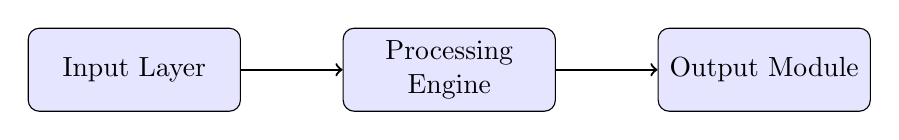
\begin{tikzpicture}[node distance=2cm, auto,
        block/.style={rectangle, draw, fill=blue!10, text width=7em, text centered, rounded corners, minimum height=3em},
        line/.style={draw, -latex', thick}]
        \node [block] (input) {Input Layer};
        \node [block, right of=input, node distance=4cm] (process) {Processing Engine};
        \node [block, right of=process, node distance=4cm] (output) {Output Module};
        \path [draw, ->, thick] (input) -- (process);
        \path [draw, ->, thick] (process) -- (output);
    \end{tikzpicture}
    \caption{Overview of System Architecture}
    \label{fig:sample_architecture}
    \source{Author's design}
\end{figure}

As shown in Figure~\ref{fig:sample_architecture}, data flows sequentially through the three main stages.

% ================= SECTION 3.2 =================
\section{Component Specifications}
\label{sec:specifications}

Table~\ref{tab:sample_specifications} summarizes the system module specifications.

\begin{table}[H]
    \caption{Module Specifications and Functional Roles}
    \label{tab:sample_specifications}
    \centering
    \begin{tabular}{|l|p{6cm}|p{4.5cm}|}
        \hline
        \textbf{Module Name} & \textbf{Functional Description} & \textbf{Key Technology} \\ \hline
        Input Handler & Validates and parses incoming raw requests & Parser, JSON / UTF-8 \\ \hline
        Core Processor & Executes computational and transformation logic & Algorithm Core \\ \hline
        Storage Layer & Persists results and logs intermediate states & File System / DB \\ \hline
    \end{tabular}
    \source{Author's compilation}
\end{table}
